\section{Compressed Sensing for Radio Astronomy} \label{cs}
A compressed sensing algorithm consists of three components: A Prior, an Objective and an Optimization Algorithm. 

To Include wide field imaging in the objective function directly, which has the potential to improve reconstruction with 
Model the signal to so the reconstruction is plausible
Use an optimization algorithm that is able to handle the expected amount of data. Interferometers produce a large amount of data. In this project, the optimization algorithm was not further investigated. The GuRoBi simplex solver was used.

Compressed Sensing for Radio Astronomy is an active research field. The new instrument's push to wide Field of View imaging has led to increased interest. 

The guarantees in Compressed Sensing depend on the signal, in what space the signal is measured and how well our Prior models the signal. 


\subsection{Sparseland Prior and Incoherence}
From compression algorithm, we assume there is a Prior $P$ in which our signal can be sparsely represented. It is not guaranteed that such a space exists, but for natural signals there always seem to be. This has led to the idea of the Sparseland Prior \eqref{cs:eq:sparseDic}: We assume for our signal there exists a Dictionary $Dic$ of signal parts. There is potentially a large, but finite number entries of parts. When we measure our signal $x$, we see a combination of only a few entries non-zero entries $\alpha$ of the Dictionary. 

\begin{equation} \label{cs:eq:sparseDic}
	\begin{split}
		x = Dic \: \alpha  \qquad  x \in \mathbb{R}^{n}, \alpha \in \mathbb{R}^{m}, Dic \in \mathbb{R}^{n*m}, \qquad n \leq m \\
		\left \| \alpha \right \|_0 = s \qquad s \ll n \leq m
	\end{split}
\end{equation}

In image compression this phenomenon was already observed: image depicting nature scenes tend to be sparse in the wavelet domain. . If $x$ in \eqref{cs:eq:sparseDic} are nature scenes, we can create a Dictionary $Dic$ of wavelets. A single image $x$ can be represented with a few wavelets, meaning the number of non-zero entries $s$ in $\alpha$ is far lower than the number of pixels $n$. All that is left to do for compression is save the non-zero entries of $\alpha$.

Noise tends to affect all entries of the Dictionary. Sparseland Prior has had success in image de-noising.

The signal parts is not restricted to be in one domain. It can consists of wavelets, cosine functions, a combination of both, or any other function. 

Work with over-complete dictionaries, where the number of pixels $n$ is far smaller than the number of signal parts $m$. There are redundant entries which is OK, as long is it is not too redundant. There is a tradeoff in practice in how sparse a signal can be represented and how redundant the dictionary is.

Back to the ill-posed inverse problem of interferometry. Nyquist Shannon Sampling Theorem requires that if we want an image of $n$ pixels, we need at least $2n$ measurements. The small Field of View Interferometer measures complex visibilities, so for $n$ fully sampled pixels we need $n$ complex Visibility measurements.

But when we know it is a Sparseland signal and we know the Dictionary, we could try to measure in the Dictionary space, so we could try to retrieve the non-zero components and only measure $s$ samples. Sadly, this is only possible if we know which entry of the dictionary are non-zero beforehand, which is in general not possible. So we would measure different $\alpha$ and are more likely to hit a zero component. Note however that if we measure a non-zero component of $\alpha$, we learn a lot more about our signal than when we hit a zero component. So the next question is, can we measure in a space where we learn more about the non-zero components of $\alpha$?

Surprisingly, the answer is yes, there is a way. The space in which we measure our signal $x$ should be incoherent from our Dictionary. With that we maximize the amount we learn about the non-zero components of $alpha$ with each measurement. Interestingly enough, constructing an incoherent measurement space is easy: Random projections are very good at being incoherent from the dictionary. 

Random Projections are not possible, the Interferometer measures complex visibilities. Antenna configuration could help. But luckily what also can help is the Wide Field imaging. McEwen \cite{mcewen2011compressed} showed the theoretical improvement on synthetic data.

How many samples are now needed? 

CS does not need an over-complete dictionary. It can also work for wavelet domains. overcomplete dictionaries give more freedom in representation.

$P$ in our original objective function. $Dic = P^{-1}$. So if the conversion from image space to Sparseland is only defined when the dictionary is a square matrix. When it has as many signal parts as pixels. The Objective Function can be modified to work with over-complete dictionaries.


\subsection{Objective Function}
The Compressed Sensing CLEAN objective function \eqref{intro:eq:csclean} uses the L0 norm for it's regularization term, which means the Objective Function is not convex. There are specialized solvers for the L0 compressed sensing. The L1 relaxation however is practically guaranteed to have the same minimum as the L0 norm and results in a convex objective function. Since GuRoBi works better on the L1 relaxation it was chosen for this project.

As for the objective function, there are three different spaces in which one might want to reconstruct: The analysis method, where the image $x$ is minimized directly, the synthesis method where the sparse vector $\alpha$ is minimized, or by in-painting the missing Visibilities $V_2$.

\begin{alignat*}{2}
	analysis:\qquad \underset{x}{minimize} \:& \left \| D_{dirty} - x \star PSF \right \|_2^2 &&+  \lambda \left \| Px \right \|_1 \\
	synthesis:\qquad \underset{\alpha}{minimize} \:& \left \| D_{dirty} - Dic \: \alpha \star PSF \right \|_2^2 &&+ \lambda \left \| \alpha \right \|_1 \\
	in-painting:\qquad \underset{V_2}{minimize} \:& \left \| D_{dirty} - F^{-1} M V_2 \right \|_2^2 &&+ \lambda \left \| PF^{-1}V_2\right \|_1
\end{alignat*}

All three objective functions have the same global minimum. For the second and third objective $x$ can be retrieved by $x = Dic\:\alpha$ and by $x = F^{-1}V_2$ respectively. [Empirical and theoretical studies have shown an advantage of the analysis objective over the other two \cite{something}]. 

However practical considerations play a factor. $Px = \alpha$ is only true $P$ is an orthogonal transformation like the wavelet transform. Over-complete dictionaries would result in $P \in \mathbb{R}^{m*n}, n \ll m$ and may not produce a suitably sparse vector $\alpha$. Therefore over-complete prior tend to use the synthesis objective, since it only requires a transformation from sparse to image space($x = Dic\:\alpha$).

It is a similar story with in-painting: the transformation $Px2$ may be eaier represented in the fourier space, especially when $P$ contains a convolution.

The strength of Compressed Sensing is that the objective can be modified for the measurement equation, while the Optimization Algorithm and the Prior stay the same. The above objective functions represent the deconvolution problem which is only true for small Field of View imaging. 

Either A- and W-Projections are used to transform the wide FoV measurement equation \eqref{radio:eq:ftSphere} back to the deconvolution. Or the measurement equation \eqref{radio:eq:ftSphere} gets included in the data term, resulting in the new objective \eqref{cs:eq:wfield}.

\begin{equation}\label{cs:eq:wfield}
	\underset{x}{minimize} \: \left \| V - MF_{wFOV}^{-1}x \right \|_2^2 + \lambda \left \| Px\right \|_1
\end{equation}

A lot of freedom to choose. 

For this project CASA was used, which limits the choices.


\subsubsection{Implementation In Casa}
\begin{figure}[h!]
	\centering
	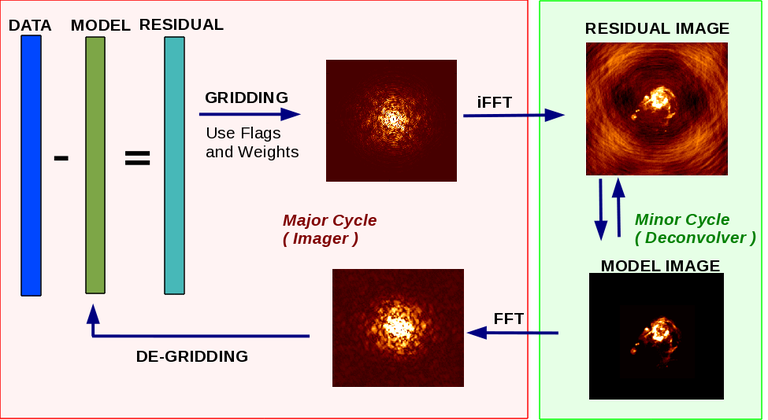
\includegraphics[width=0.6\linewidth]{./chapters/04.cs/img/casa_major_minor.png}
	\caption{Casa Major Minor Cycle, source \cite{casa2018major}}
	\label{cs:major}
\end{figure}

Casa major and minor cycle. Major cycle calculates visibilities in image space. Minor Cycle Deconvolves the Problem, often with a CLEAN class Algorithm. This constrains the algorithm to use the data term in image space. 

This forces the objective function to either minimize in the image domain or in the sparsity domain.


\subsection{Compressed Sensing Algorithms in Astronomy}

\subsubsection{SASIR}

\subsubsection{PURIFY}

\subsubsection{Vis-CS}


 
